% !TEX root = ../main.tex

\chapter{Introduction}
\label{chap:intro}
After a period of incredible advances in processing power in the Eighties, Nineties and early 2000s, progress in the field of classical single core CPUs has slowed considerably in the last 10 years. Given the ever increasing complexity of modern computer programs, different solutions had to be found. Once single core performance could not be increased at a sufficient speed anymore, the tendency to execute code in parallel arose instead. For example, modern CPUs usually have at least two cores, a lot of them even four or more. This trend is no longer specific to traditional computers such as PCs and servers, but can also be found on mobile devices such as smart phones and tablets. \\

There are two different ways to parallelize applications, i.e. task and data parallelism. Task parallelism is an instance of coarse-grained parallelism. Multiple components of the program are run concurrently, each executing its own instructions and following its own control flow. Multiple CPU cores are the prime example for the facilities that task parallel programs are executed on. Data parallelism usually denotes a more fine-grained approach to parallelism where the same instructions are executed on multiple data elements. These kind of instructions are called \textbf{S}ingle \textbf{I}nstruction \textbf{M}ultiple \textbf{D}ata (SIMD) instructions. For example, with the Intel AVX vector extensions, it is possible to  multiply a vector of eight 32 bit integer values component-wise with another, in one instruction. In applications that need to have the same operation applied on large amounts of data, this can save a considerable amount of time. \\ 

One of the most remarkable developments in the last two decades is the Graphics Processing Unit (GPU). Starting off as a simple I/O device to display two dimensional content on the computer screen, it evolved with the ever increasing demand of graphical applications. Graphical applications typically require the same operation (like for example a shader) to be executed on a large chunk of data, such as a texture file. To fulfill these requirements and satisfy the ever increasing performance demands, GPUs evolved into powerful, massively parallel processors. Due to the nature of the applications, the parallelism of GPUs is data parallel. \cite{blythe2008rise,jalili2010simd} \\

Video games are good examples of these increasingly complex graphical applications. Figure \ref{fig:intro_videogamecomp} shows two computer games, \textit{Tomb Raider II} from 1997 and \textit{Assassin's Creed IV} from 2013. They are an example for the performance gains that have been achieved in the last two decades. Today shaders are used to create realistic lighting and water effects, in the early 2000s, programming GPUs was difficult, and developers had to use tricks such as executing multiple passes to get the required results. With the introduction of the Pixel and Vertex shader, people started writing general purpose code for the GPU. Writing general purpose code for these shaders was possible, but difficult. One had to write the shader as if it were displayed, then extract the result from the device's memory. \cite{jalili2010simd,blythe2008rise} \\

\begin{figure}
  \centering
  \begin{subfigure}{.4\textwidth}
      \centering
      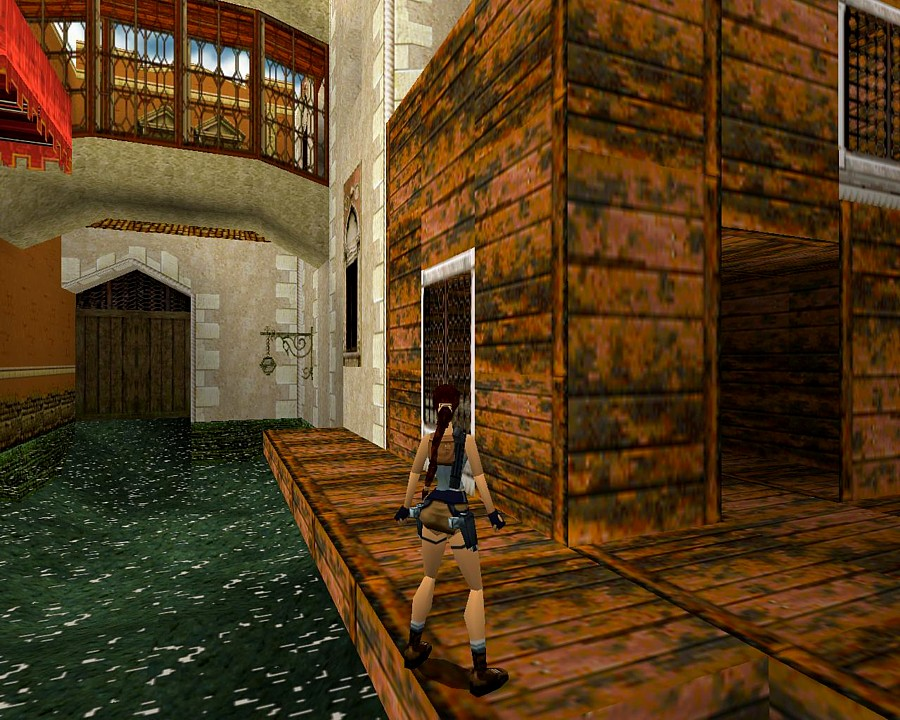
\includegraphics[width=.95\linewidth]{images/oldGraphics}
      \caption{Tomb Raider II (1997)}
      \label{fig:intro_tomb}
  \end{subfigure}
  \begin{subfigure}{.55\textwidth}
      \centering
      
\includegraphics[width=.95\linewidth]{images/modernGraphics}
      \caption{Assassin's Creed (2014)}
      \label{fig:intro_assassin}
  \end{subfigure}
  \caption{Comparison of complexity of video game graphics. Modern GPUs can display graphics that are more complex, by several orders of magnitude.}
  \label{fig:intro_videogamecomp}
\end{figure}

Some years later, Pixel and Vertex shader units were unified into more general purpose unified Shader units, and around the same time the term of General Purpose GPU (GPGPU) Computing came into use. Microsoft introduced the DirectCompute API, NVidia the CUDA API and the Khronos Group the OpenCL API to enable developers to move parts of the execution of their programs to the GPU. All of these APIs enabled the programmer to execute general purpose code on the GPU without having to use facilities and APIs designed to display graphics. All of them use a C like language that is compiled for the individual GPUs at run time. \cite{khronos2008release,khronos2012specification,nvidia2009opencl} \\
\newpage



%%%%%%%%%%%%%%%%%%%%%%%%%%%%%%%%%%%%%%%%%%%%%%%%%%%%%%%%%%%%%%%
\section{Motivation}
\label{sect:intro_motivation}

Code executed in such a matter can be significantly faster than normal sequential code, especially if it is heavy on computations. Unfortunately, there is a rather high overhead, as resources need to be transferred to the device\footnote{The computing device used, for example the GPU of the PC.}. Figure \ref{fig:intro_performance_cpu_gpu} compares the execution time of applying an operation on every element of a two-dimensional array, with different sizes, using conventional methods and with the execution using a GPU and OpenCL. The first thing one notes is that the overhead alone makes it not viable to perform kernels on the GPU for small arrays. For these arrays, in this example those with less than about $5*10^4$ elements, the time spent on copying alone is larger than just executing the whole computation conventionally using the CPU. For larger arrays, there is a significant benefit to performing the computation on the GPU. This is especially true when comparing just the execution of the operation. If there is more then one operation that is performed on the GPU, and the data is already on the GPU, then the difference in execution time is about a single order of magnitude.\\

\begin{figure}[h]
  \begin{center}
    \begin{tikzpicture}
      \begin{loglogaxis}[ xlabel=Number of Elements, 
              ylabel=Time in µs,
              legend entries={CPU Total, GPU Total, GPU Execution},
              legend style={at={(1.03, 0.5)}, anchor=west}]
        \addplot [red, error bars/.cd, y dir=both, y explicit] table [x=elements, y=cpu, y error=cpuStdDev]{data/cpugpu.csv};
        \addplot [blue, error bars/.cd, y dir=both, y explicit] table [x=elements, y=gpu, y error=gpuStdDev]{data/cpugpu.csv};
        \addplot [green, error bars/.cd, y dir=both, y explicit] table [x=elements, y=run, y error=runStdDev]{data/cpugpu.csv};
      \end{loglogaxis}
    \end{tikzpicture}
    \caption{Execution time for the execution of a kernel with different number of elements. The red graph shows the time spent on executing the kernel on the CPU, using parallel for loops and vectorization. The blue graph shows the total execution time for the GPU, including the transfer of the memory to and from the device. The green graph shows the time spent executing the kernel on the GPU.}
    \label{fig:intro_performance_cpu_gpu}
  \end{center}
\end{figure}

There are, however, some downsides to executing code on the GPU. There is still a great amount of boilerplate code involved when writing OpenCL code. A lot of repetitive calls to C APIs need to be made, memory needs to be managed manually, work-group sizes determined and kernels enqueued for execution. Additionally, it may not always be a good idea to outsource the computation. OpenCL has certain restrictions, and is not suited for every kind of computation. Additionally, as seen above, there might not even always be a performance benefit. This thesis is part of an effort to address these concerns by implementing a compiler that automatically generates code both for the CPU and the GPU\footnote{See chapter \ref{chap:compiler}}, and selects the right kind of execution based upon the available resources and the program that is executed. Deciding whether to execute a computation on the GPU requires knowledge about the costs that come with the execution. Chapter \ref{chap:model} presents such a model. 